\section{Introduction}
\label{sec:introduction} 

On-policy distillation (OPD)~\citep{AgarwalVZSGGB24,Gu0WH24,abs-2505-09388,abs-2512-02556,lu2025onpolicydistillation,abs-2601-18734} transfers capabilities from a stronger teacher to a student large language model (LLM) by minimizing token-level KL divergence on student-generated rollouts. By supervising contexts induced by the student's own policy, OPD reduces the train--inference mismatch and provides dense token-level guidance, in contrast to the typically sparse outcome-level rewards of reinforcement learning with verifiable rewards (RLVR), leading to promising results on complex tasks such as mathematical reasoning~\citep{lu2025onpolicydistillation,abs-2603-07079}. Extending OPD to multi-turn agentic tasks~\citep{abs-2409-12122,ShridharYCBTH21}, however, introduces a trajectory drift challenge: because each action shapes subsequent observations, an incorrect tool call, or even a valid action unlikely under the teacher policy, can lead the student into \emph{off-teacher-distribution states} rarely encountered in teacher-generated rollouts~\citep{abs-2605-07725,abs-2604-24005}, as illustrated in \Cref{fig:intro}. As such deviations accumulate across turns, teacher--student policy discrepancy can increase, making the teacher's token-level guidance on the resulting histories less reliable or even counterproductive~\citep{abs-2604-13016}. Consequently, supervising student-generated tokens alone may be insufficient to control the distribution shift induced by multi-turn interaction. 



Existing methods address this instability through two strategies.
One masks or reweights the distillation loss using signals derived from KL divergence~\citep{abs-2605-07725,abs-2606-19659} or model confidence~\citep{abs-2604-10688}.
The other controls training-trajectory construction by progressively adjusting rollout depth~\citep{abs-2604-24005} or mixing teacher- and student-generated turns through a curriculum~\citep{abs-2606-15912}.
However, loss filtering will lose supervision signals and cannot directly correct the action that determines the next environment transition.
Predefined curricula and rollout-depth control can prevent the student's exposure to unreliable supervision, but do not adaptively assess whether its current response requires correction.
Recent work has further explored \emph{teacher intervention} that allows the teacher to take over from the students' generation at specific points~\citep{abs-2607-26057}. 
By replacing the student's proposed action with a teacher-generated one, these methods could limit the accumulation of trajectory drift and provide more reliable supervision on subsequent turns. 



However, making teacher intervention effective in multi-turn OPD still requires addressing two key challenges.
First, \emph{\textbf{when should the teacher intervene?}}
Predefined intervention schedules fail to account for immediate changes in teacher--student policy discrepancy during multi-turn interactions~\citep{abs-2606-15912}. 
On the other hand, recent adaptive approaches use discrepancy estimates to guide intervention through decision boundaries, hysteretic thresholds, or lookahead validation~\citep{abs-2605-19433,abs-2607-29078,abs-2608-01953}. 
However, these estimates are subject to statistical noise, and threshold-based decisions can amplify estimation errors into abrupt changes in teacher control.
A poor intervention strategy may therefore miss opportunities to correct trajectory drift or intervene unnecessarily, increasing teacher dependence and computational cost. 
\begin{wrapfigure}{l}{0.6\textwidth}
    \centering
    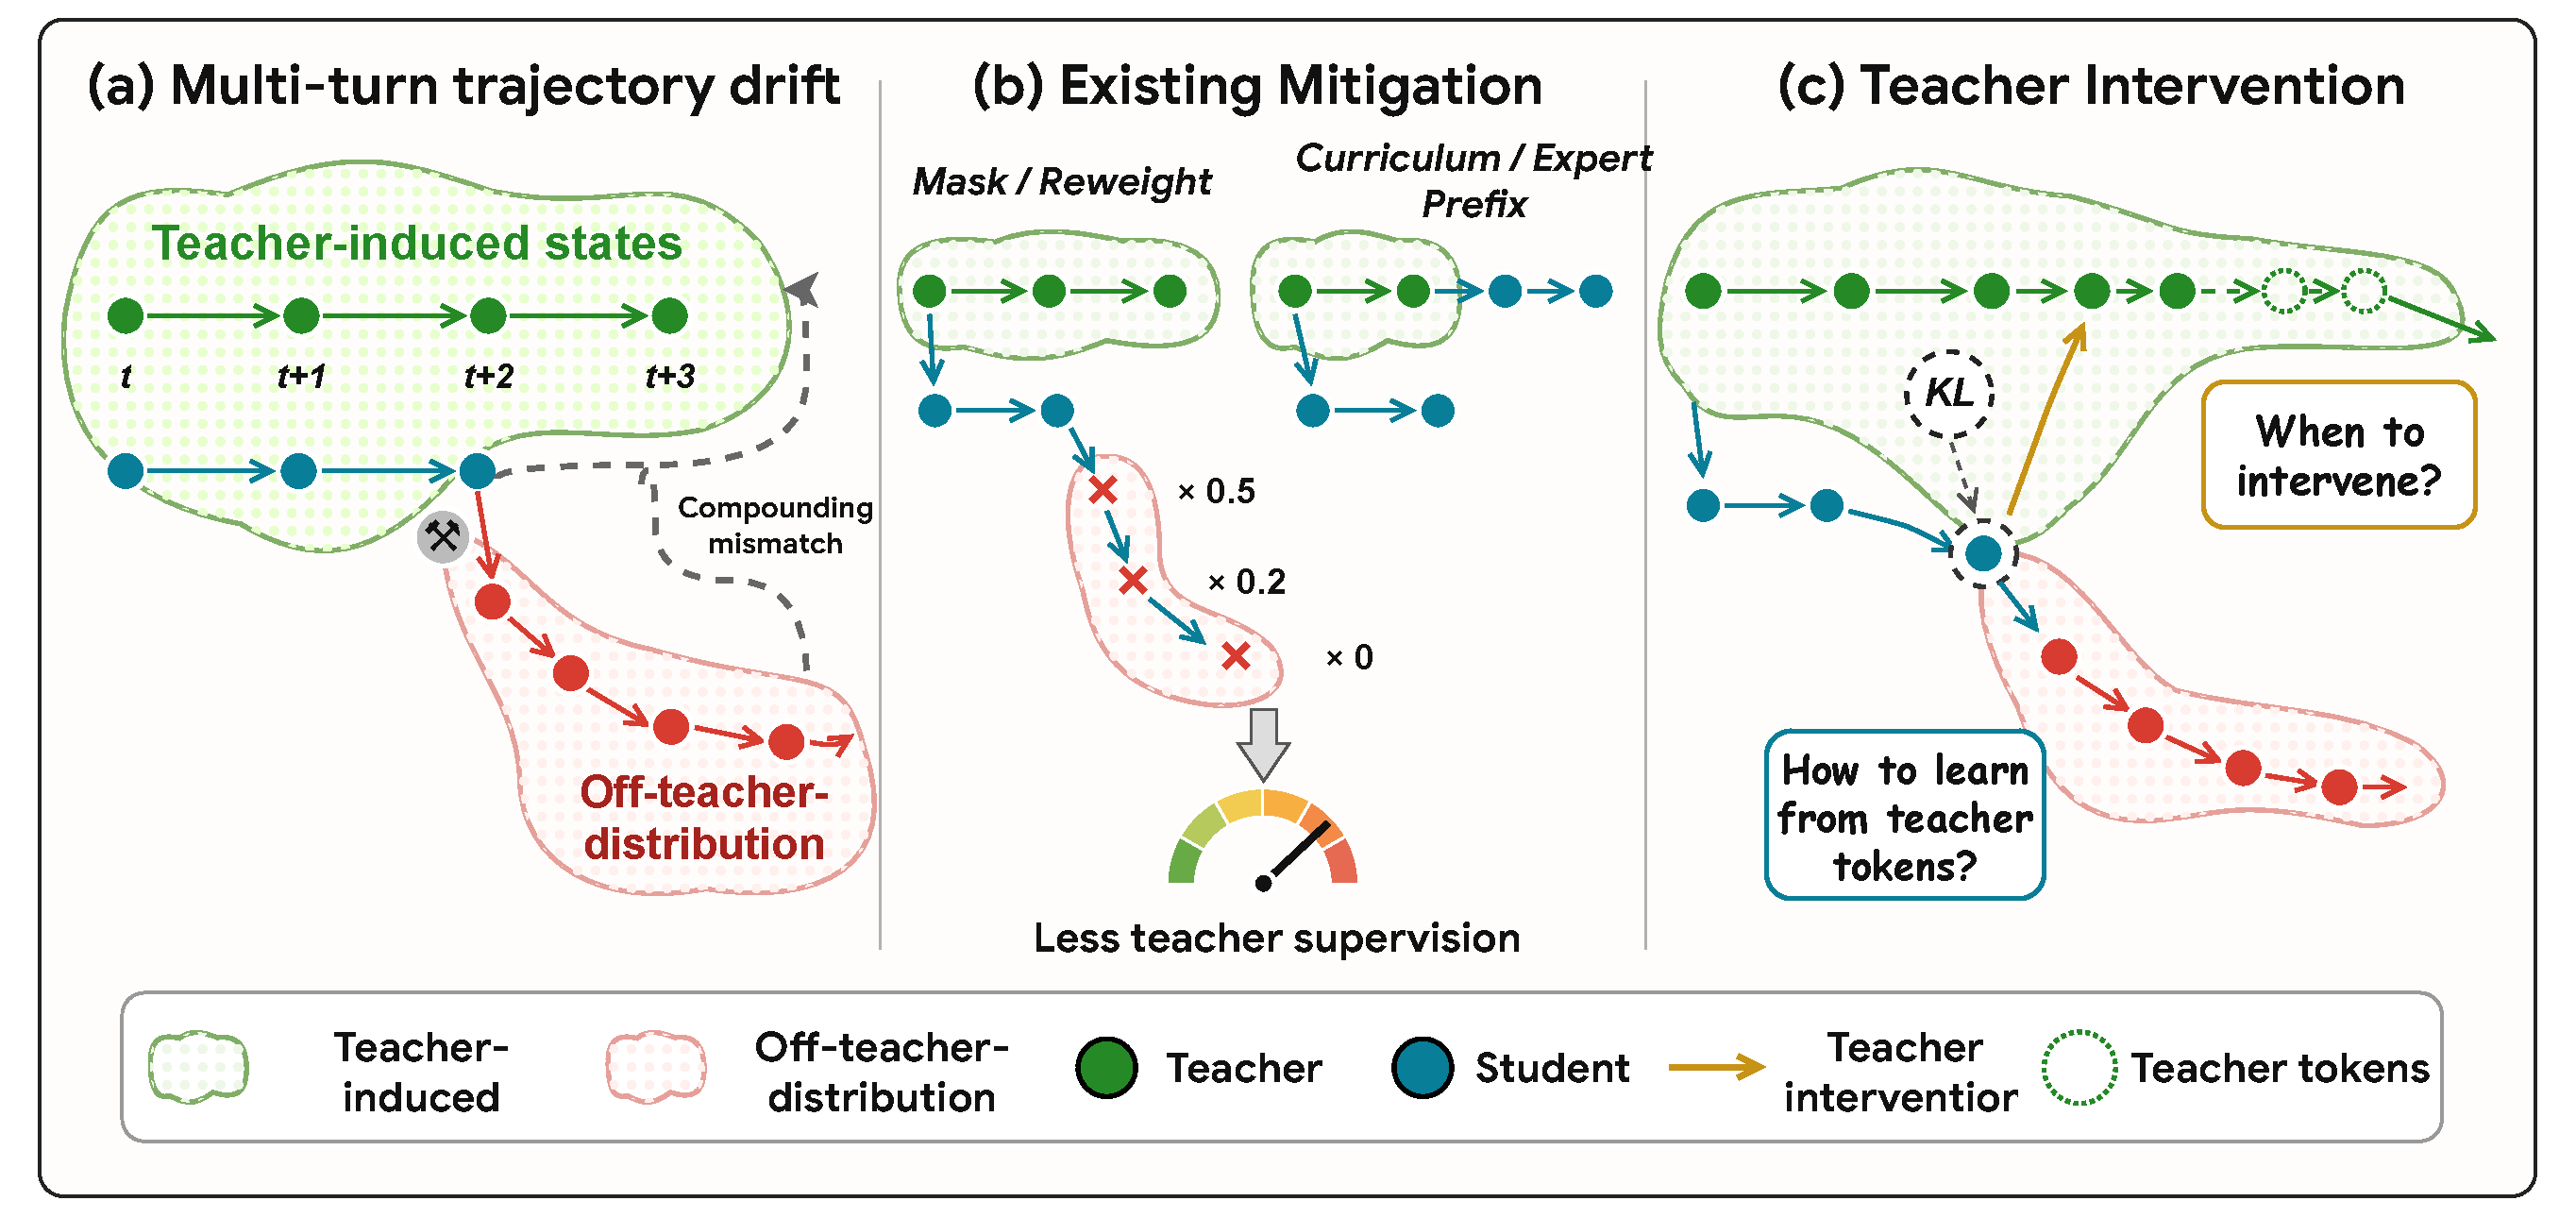
\includegraphics[width=.6\textwidth]{figs/introv2.pdf}
    \caption{Illustration of trajectory-level distribution shift and turn-level teacher intervention in on-policy distillation.}
    \label{fig:intro}
    \vspace{-1.0em}
\end{wrapfigure} 
Second, \emph{\textbf{how should the student learn from teacher-generated tokens?}}
Teacher intervention introduces tokens sampled from the teacher policy into training, whereas standard OPD defines its reverse-KL objective under student-generated tokens.
Existing intervention-based OPD methods handle these teacher-generated tokens using different surrogate objectives~\citep{abs-2606-15912,abs-2607-26057,abs-2608-01953}.
Some adopt forward-KL or SFT-style objectives, which depart from the reverse-KL formulation of standard OPD and may affect the retention of previously acquired capabilities.
Others directly apply a sampled reverse-KL objective to teacher-generated tokens.
However, because these tokens are sampled from the teacher rather than the student policy, directly evaluating the standard reverse-KL integrand does not recover its intended expectation under the student policy.
Thus, learning from teacher intervention requires correcting this token-sampling mismatch while preserving the conditional reverse-KL objective of OPD.


To address these challenges, we propose \name, a discrepancy-guided \underline{S}tochastic \underline{T}eacher \underline{I}ntervention framework for multi-turn agentic OPD.
We first develop a stochastic intervention strategy that samples whether to intervene based on teacher--student policy discrepancy. 
Specifically, \name uses KL divergence estimated by $k_3$ estimator~\citep{Schulman2020KL} to measure the divergence between the teacher and student policies at each turn, and maps this estimate into an intervention probability.
This probability increases smoothly with the discrepancy, favoring teacher intervention when the policies diverge while preserving student exploration, without a hand-tuned threshold or fixed intervention budget.
To learn from the resulting mixed-policy trajectories, we further introduce an importance-weighted reverse KL objective that uses importance sampling~\citep{SchulmanWDRK17} to correct the token sampling mismatch between teacher-generated responses and the student policy while preserving the original OPD objective formulation.
Intervention thus controls which histories are visited, while importance weighting corrects the token-sampling mismatch introduced by teacher generation. 

Extensive experiments are conducted in two multi-turn agentic settings, spanning tool-integrated reasoning~\citep{aime24,aime25,aime26,abs-2605-00674,abs-2311-12022,JainHGLYZWSSS25} and long-horizon agentic interaction~\citep{ShridharYCBTH21,WangJCA22}.
\name outperforms all distillation baselines on each benchmark and at both student scales, with its largest margins on long-horizon tasks, where compounding error is most severe. 
Ablations show that different components of \name contribute to these gains and further analysis reveals the mechanism, scalability, and efficiency of \name. 

